\documentclass[12pt,addpoints,answers]{exam}
\usepackage[utf8]{inputenc}

\unframedsolutions
\renewcommand{\solutiontitle}{\noindent\textbf{Solution:}\par\noindent}
\SolutionEmphasis{\color{blue}}
%\noprintanswers

\usepackage{booktabs}
\usepackage{tabularx}
\usepackage{url}
\usepackage{xfrac}

\usepackage{siunitx}
\sisetup{parse-numbers=false}

\usepackage{listings}
\lstset{basicstyle=\scriptsize\ttfamily}

\usepackage{tikz}
\usetikzlibrary{arrows}
\usetikzlibrary{decorations.pathreplacing}
\usetikzlibrary{chains}
\usetikzlibrary{positioning}
%\tikzset{>=stealth',every on chain/.append style={join}, every join/.style={-,blue,thick,dashed}}

% tables
\usepackage{multirow}
\usepackage{booktabs}

\title{Computer Networks Homework 4}
\author{Spring 2020}
\date{Due: 6 April 2020}

\begin{document}
\maketitle

\begin{questions}
\question Indicate whether each of the following tasks is a responsibility of the control plane or the data plane of the Network Layer.
\begin{parts}
\part[2] Updating forwarding decisions when a link we used to transmit packets is now out of service.
\begin{solution}
	Control Plane
\end{solution}
\part[2] Building the forwarding tables in the memory of a device.
\begin{solution}
	Control Plane
\end{solution}
\part[2] Updating forwarding tables when new capacity has been added.
\begin{solution}
	Control Plane
\end{solution}
\part[2] Forwarding a packet based on the forwarding table.
\begin{solution}
	%https://networkengineering.stackexchange.com/questions/38573/difference-between-control-plane-data-plane-and-management-plane
	Data Plane
\end{solution}
\end{parts}

\question[12] Suppose a router has three input flows and one output. It receives all of the packets listed in the table below at effectively the same time $S_i = 0$ the same time, in the order listed. Assume that all flow queues are otherwise empty. Give the order in which the packets are transmitted using fair queuing.
\begin{center}
\begin{tabularx}{0.7\linewidth}{l|*8{>{\centering\arraybackslash}X}}
\toprule
\emph{Packet} &   1 &   2 &   3 &   4 &   5 &   6 &   7 &   8 \\
\emph{Size}   & 100 & 100 & 100 & 100 & 190 & 200 & 110 &  50 \\
\emph{Flow}   &   1 &   1 &   1 &   1 &   2 &   2 &   3 &   3 \\
\bottomrule
\end{tabularx}
\end{center}
\begin{solution}
	% All of these coming in at the exact same time is insane, but sure.
	% Thoughts:
	% See all 3 flows empty to begin with, start with smallest from each flow.
	% Then iterate through each flow selecting the smallest possible at that time, from when uncomsumed per flow.
	\begin{itemize}
		\item Packet 8
		\item Packet 1
		\item Packet 5
		\item Packet 7
		\item Packet 2
		\item Packet 6
		\item Packet 3
		\item Packet 4
	\end{itemize}
\end{solution}

\question[6] Give the forwarding tables for switches S1 to S4 in the following network. In addition to entries A--D, each table should also have a default routing entry, chosen to forward packets with unrecognized destination addresses towards OUT.
\begin{center}
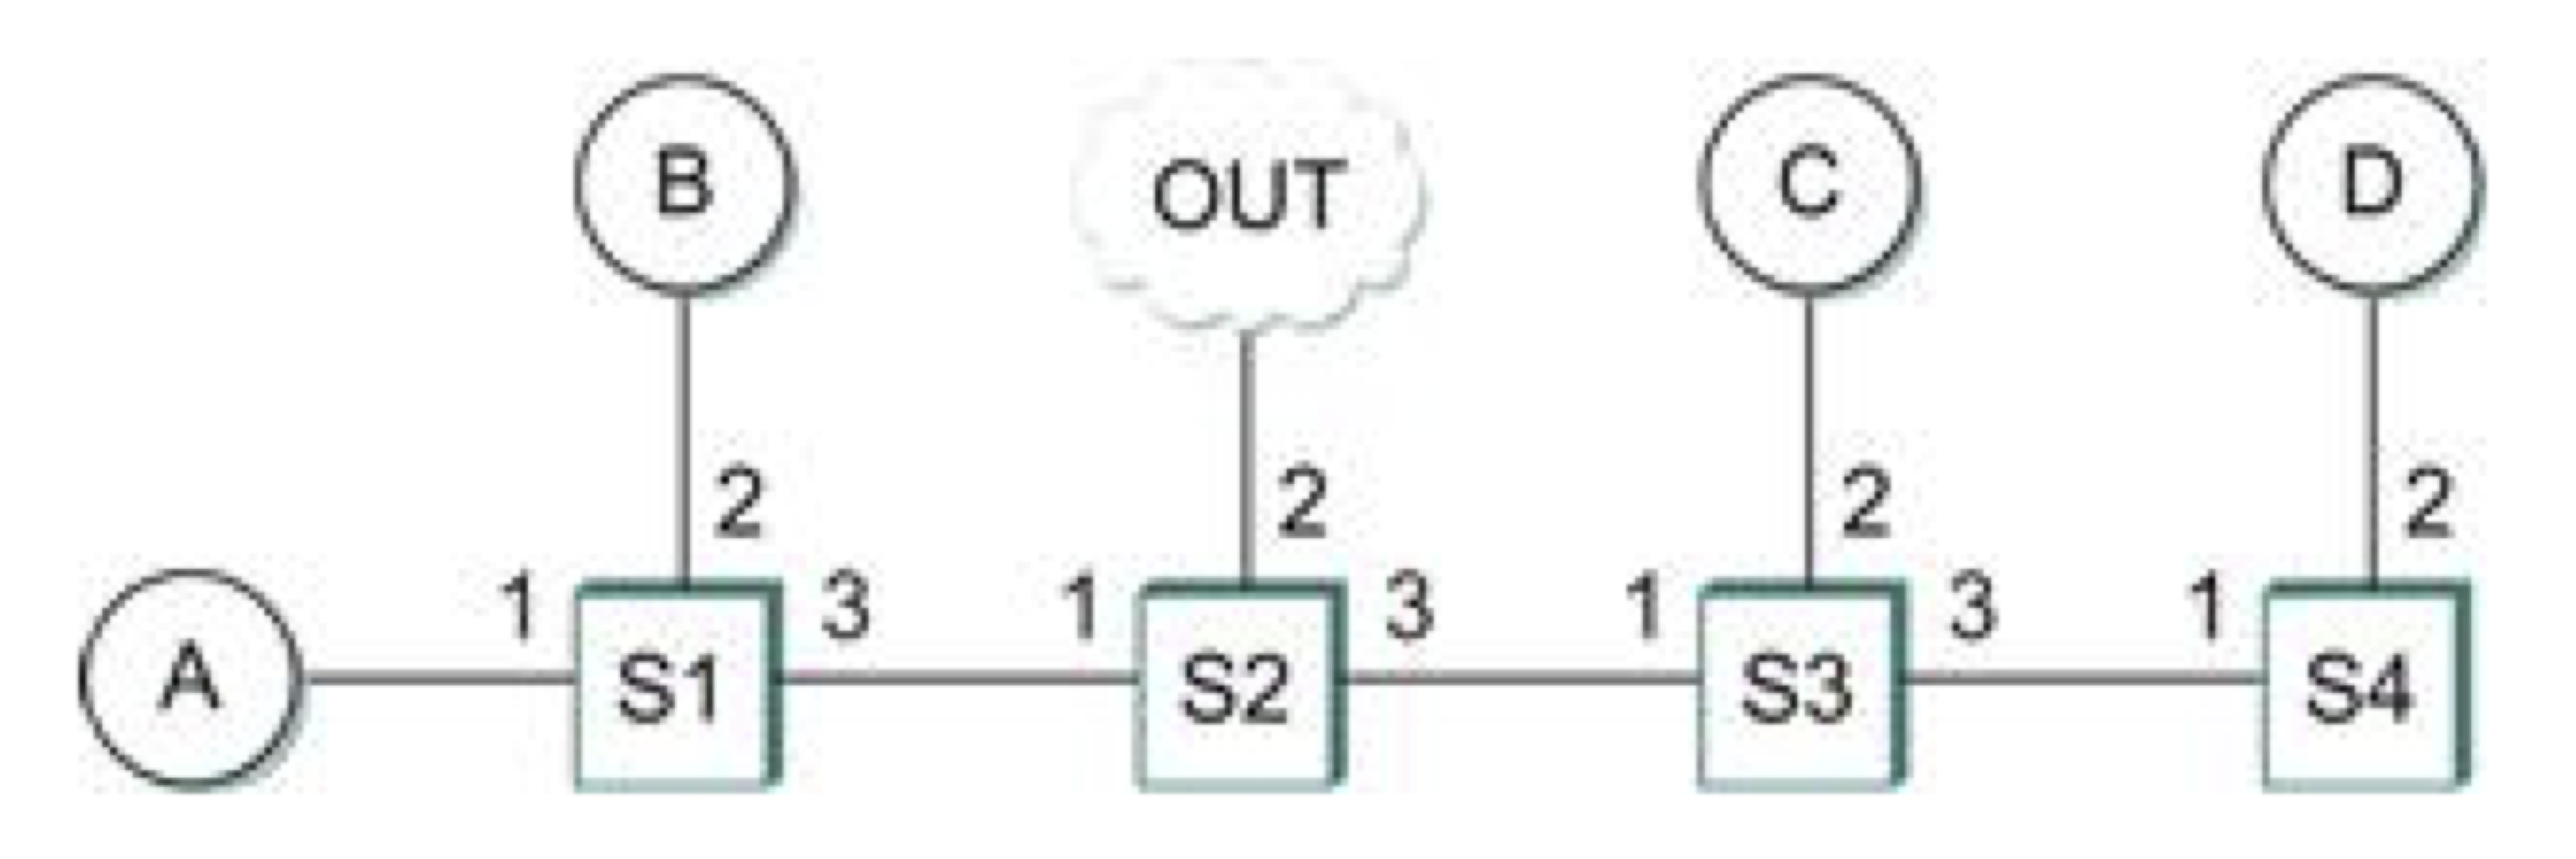
\includegraphics[width=0.6\linewidth]{fig/simple.png}
\end{center}
\begin{solution}
	See "Table 1: Solution 3" below.
	
	Weird formatting issues wouldn't allow the table to render in a solution tab due to "Float(s) lost" errors.
	\begin{table}[]
		\centering
		\caption{Solution 3}
		\label{Table 1}
		\begin{tabular}{|c|c|c|c|c|}
			\cline{1-2} \cline{4-5}
			\multicolumn{2}{|c|}{Switch \#1} & \multirow{7}{*}{} & \multicolumn{2}{c|}{Switch \#2} \\ \cline{1-2} \cline{4-5} 
			Destination      & Out Port      &                   & Destination      & Out Port     \\ \cline{1-2} \cline{4-5} 
			A                & 1             &                   & A                & 1            \\
			B                & 2             &                   & B                & 1            \\
			C                & 3             &                   & C                & 3            \\
			D                & 3             &                   & D                & 3            \\
			Unknown          & 3             &                   & Unknown          & 2            \\
			\multicolumn{5}{|c|}{}                                                                 \\ \cline{1-2} \cline{4-5} 
			\multicolumn{2}{|c|}{Switch \#3} & \multirow{7}{*}{} & \multicolumn{2}{c|}{Switch \#4} \\ \cline{1-2} \cline{4-5} 
			Destination      & Out Port      &                   & Destination      & Out Port     \\ \cline{1-2} \cline{4-5} 
			A                & 1             &                   & A                & 1            \\
			B                & 1             &                   & B                & 1            \\
			C                & 2             &                   & C                & 1            \\
			D                & 3             &                   & D                & 2            \\
			Unknown          & 1             &                   & Unknown          & 1           
		\end{tabular}
	\end{table}
\end{solution}
% Please add the following required packages to your document preamble:
% \usepackage{multirow}
\begin{table}[]
	\centering
	\caption{Solution 3}
	\label{Table 1}
	\begin{tabular}{|c|c|c|c|c|}
		\cline{1-2} \cline{4-5}
		\multicolumn{2}{|c|}{Switch \#1} & \multirow{7}{*}{} & \multicolumn{2}{c|}{Switch \#2} \\ \cline{1-2} \cline{4-5} 
		Destination      & Out Port      &                   & Destination      & Out Port     \\ \cline{1-2} \cline{4-5} 
		A                & 1             &                   & A                & 1            \\
		B                & 2             &                   & B                & 1            \\
		C                & 3             &                   & C                & 3            \\
		D                & 3             &                   & D                & 3            \\
		Unknown          & 3             &                   & Unknown          & 2            \\
		\multicolumn{5}{|c|}{}                                                                 \\ \cline{1-2} \cline{4-5} 
		\multicolumn{2}{|c|}{Switch \#3} & \multirow{7}{*}{} & \multicolumn{2}{c|}{Switch \#4} \\ \cline{1-2} \cline{4-5} 
		Destination      & Out Port      &                   & Destination      & Out Port     \\ \cline{1-2} \cline{4-5} 
		A                & 1             &                   & A                & 1            \\
		B                & 1             &                   & B                & 1            \\
		C                & 2             &                   & C                & 1            \\
		D                & 3             &                   & D                & 2            \\
		Unknown          & 1             &                   & Unknown          & 1           
	\end{tabular}
\end{table}


\newpage

\question[6] Create the forwarding table for switch 1 in the "fish" network below. How did you base your forwarding decisions?
\begin{center}
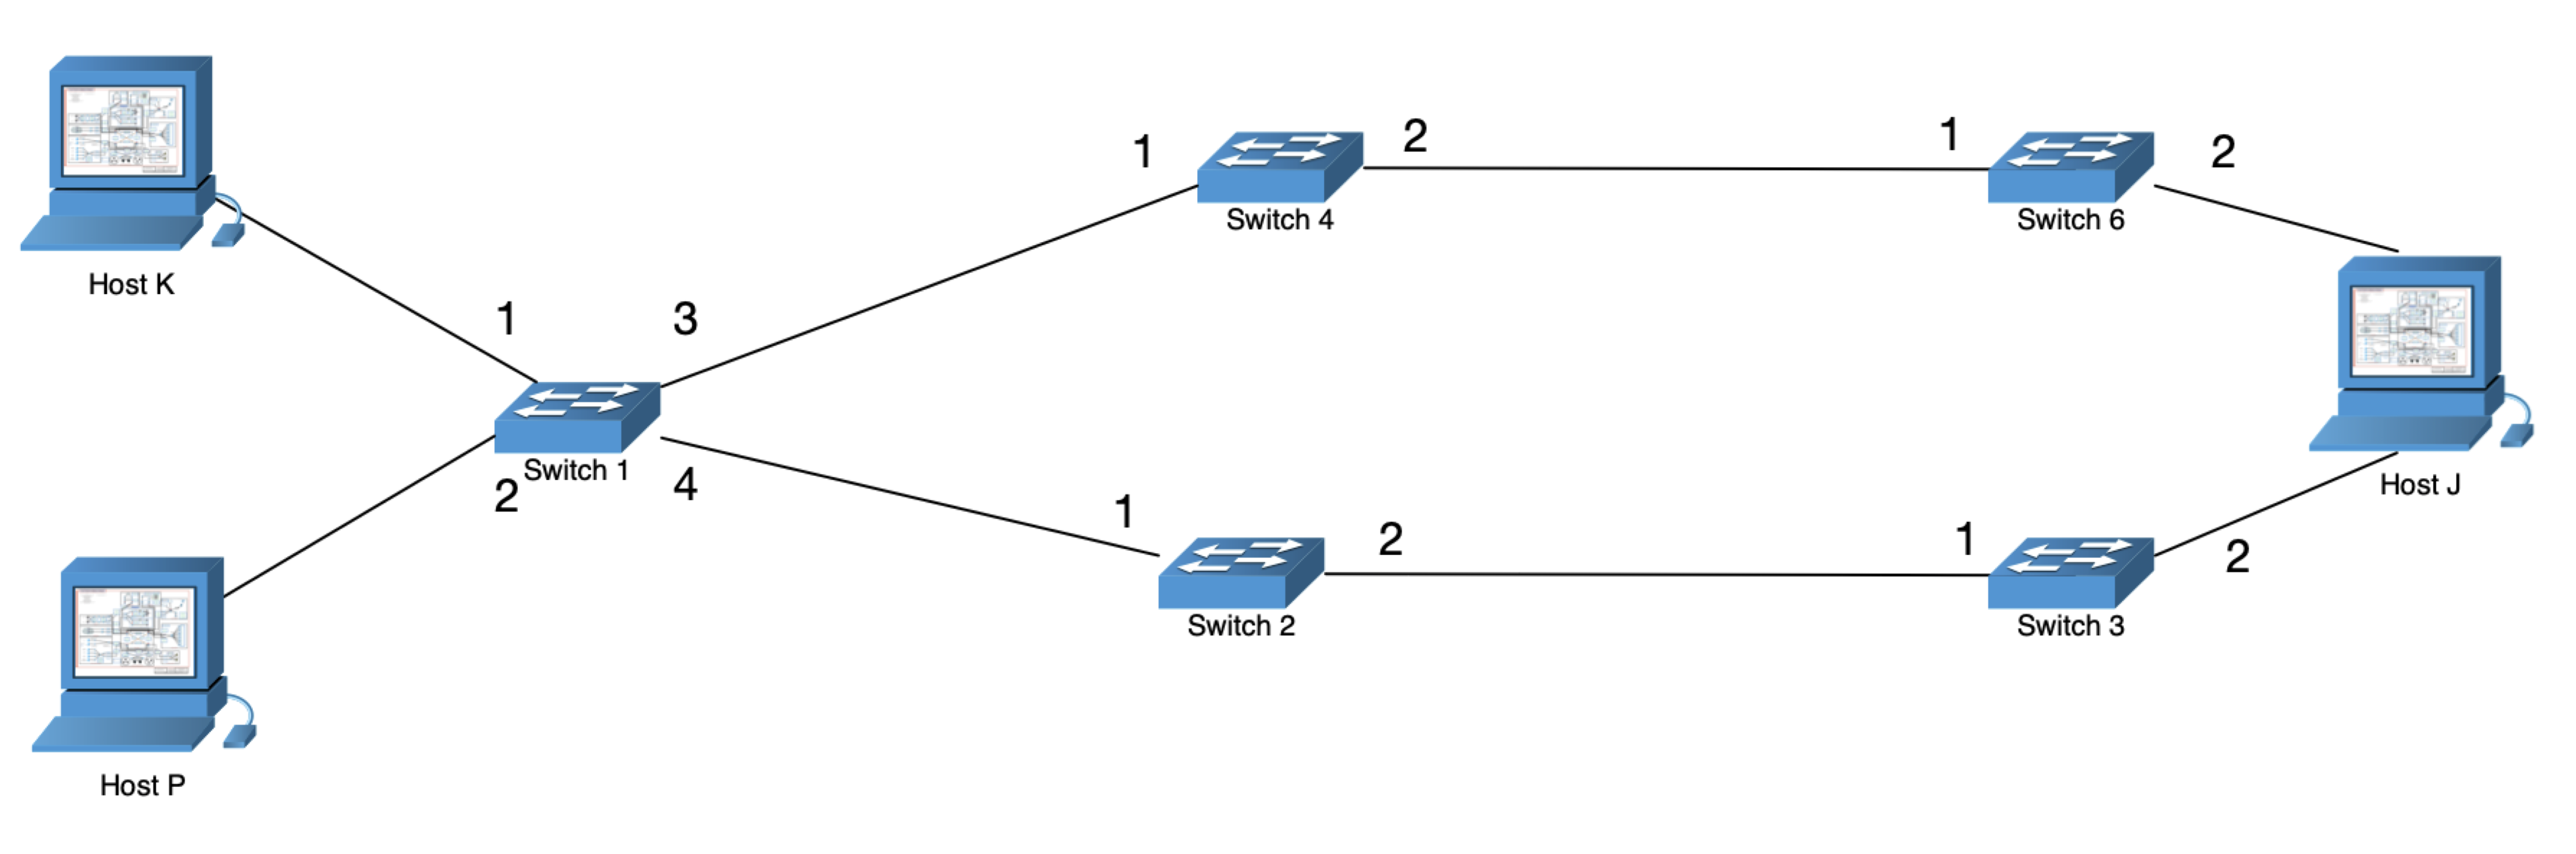
\includegraphics[width=1.0\linewidth]{fig/fish.png}
\end{center}
\begin{solution}
	See "Table 2: Solution 4" below.
	
	Weird formatting issues wouldn't allow the table to render in a solution tab due to "Float(s) lost" errors.
	
	My decision to send traffic from to hosts P and K are trivially obvious as they are the only connection available.  For Host J switch 2 (port 4) was select since it was a lower named switch and therefore should have a lower ID (by possibly common sense logic).
	
	Alternatively, another option may be to route traffic from hosts K to J along Switch 4 (port 3) and traffic from hosts P to J along switch 2 (port 4) as a form of load balancing.
\end{solution}
\begin{table}[]
	\centering
	\caption{Solution 4}
	\label{Table 2}
	\begin{tabular}{|c|c|}
		\hline
		\multicolumn{2}{|c|}{Switch \#1}      \\ \hline
		Destination Label & Destination Port \\ \hline
		Host K            & 1                \\
		Host P            & 2                \\
		Host J            & 4               
	\end{tabular}
\end{table}
\newpage

\question[4] Some signaling errors can cause entire ranges of bits in a packet to be overwritten by all 0s or all 1s. Suppose all the bits in an IP packet, including the checksum are overwritten. Using what you know about the IPv4 packet header...
\begin{enumerate}
\item Could a packet with all 0s be a legal IPv4 packet?
\item Could a packet with all 1s be a legal IPv4 packet?
\item Would the checksum catch either error?
\end{enumerate}
Recall: the IPv4 checksum is the binary complement of the one's complement sum of all 16-bit words in the header.
\begin{solution}
	\begin{enumerate}
		\item No
		\item No
		\item Wouldn't need to
	\end{enumerate}
	
	If the entire packet range is entirely overwritten with all 0's or 1's then the version field would either be 0 or 16 neither of which exist and should be instant grounds for throwing away the packet as illegitimate as how to parse the rest of it becomes a mystery.  
\end{solution}

\question[8] Suppose a TCP message that contains 1024 bytes of data and the 20 byte TCP header is passed to IP for delivery across two networks interconnected by a router (i.e., it travesl from the source host to a router, and then from the router to the destination host). The first network has an MTU of 1024 bytes; the second has an MTU of 576 bytes. Give the sizes and offsets of each packet that arrives at the network layer of the destination host, keeping in mind that the network may have to fragment the packets. You should assume that all IP headers are 20 bytes.
\begin{solution}
	To Switch from Host:
	\begin{enumerate}		
		\item Packet 1: 
		\begin{enumerate}
			\item Size: 1004 + 20 bytes for IP Header
			\item Offset: 0
		\end{enumerate}
			\item Packet 2: 
		\begin{enumerate}
			\item Size: 20 + 20 bytes for IP Header
			\item Offset: 1004
		\end{enumerate}
	\end{enumerate}

	To Host from Switch:
	\begin{enumerate}	
	\item Packet 1: 
	\begin{enumerate}
		\item Size: 556 + 20 bytes for IP Header
		\item Offset: 0
	\end{enumerate}
	\item Packet 2: 
	\begin{enumerate}
		\item Size: 448 + 20 bytes for IP Header
		\item Offset: 556
	\end{enumerate}
	\item Packet 3:
	\begin{enumerate}
		\item Size: 20 + 20 bytes for IP Header
		\item Offset: 1004
	\end{enumerate}
\end{enumerate}
\end{solution}

\question For the following network, give the global distance vector tables at each of the following time steps.
\begin{center}
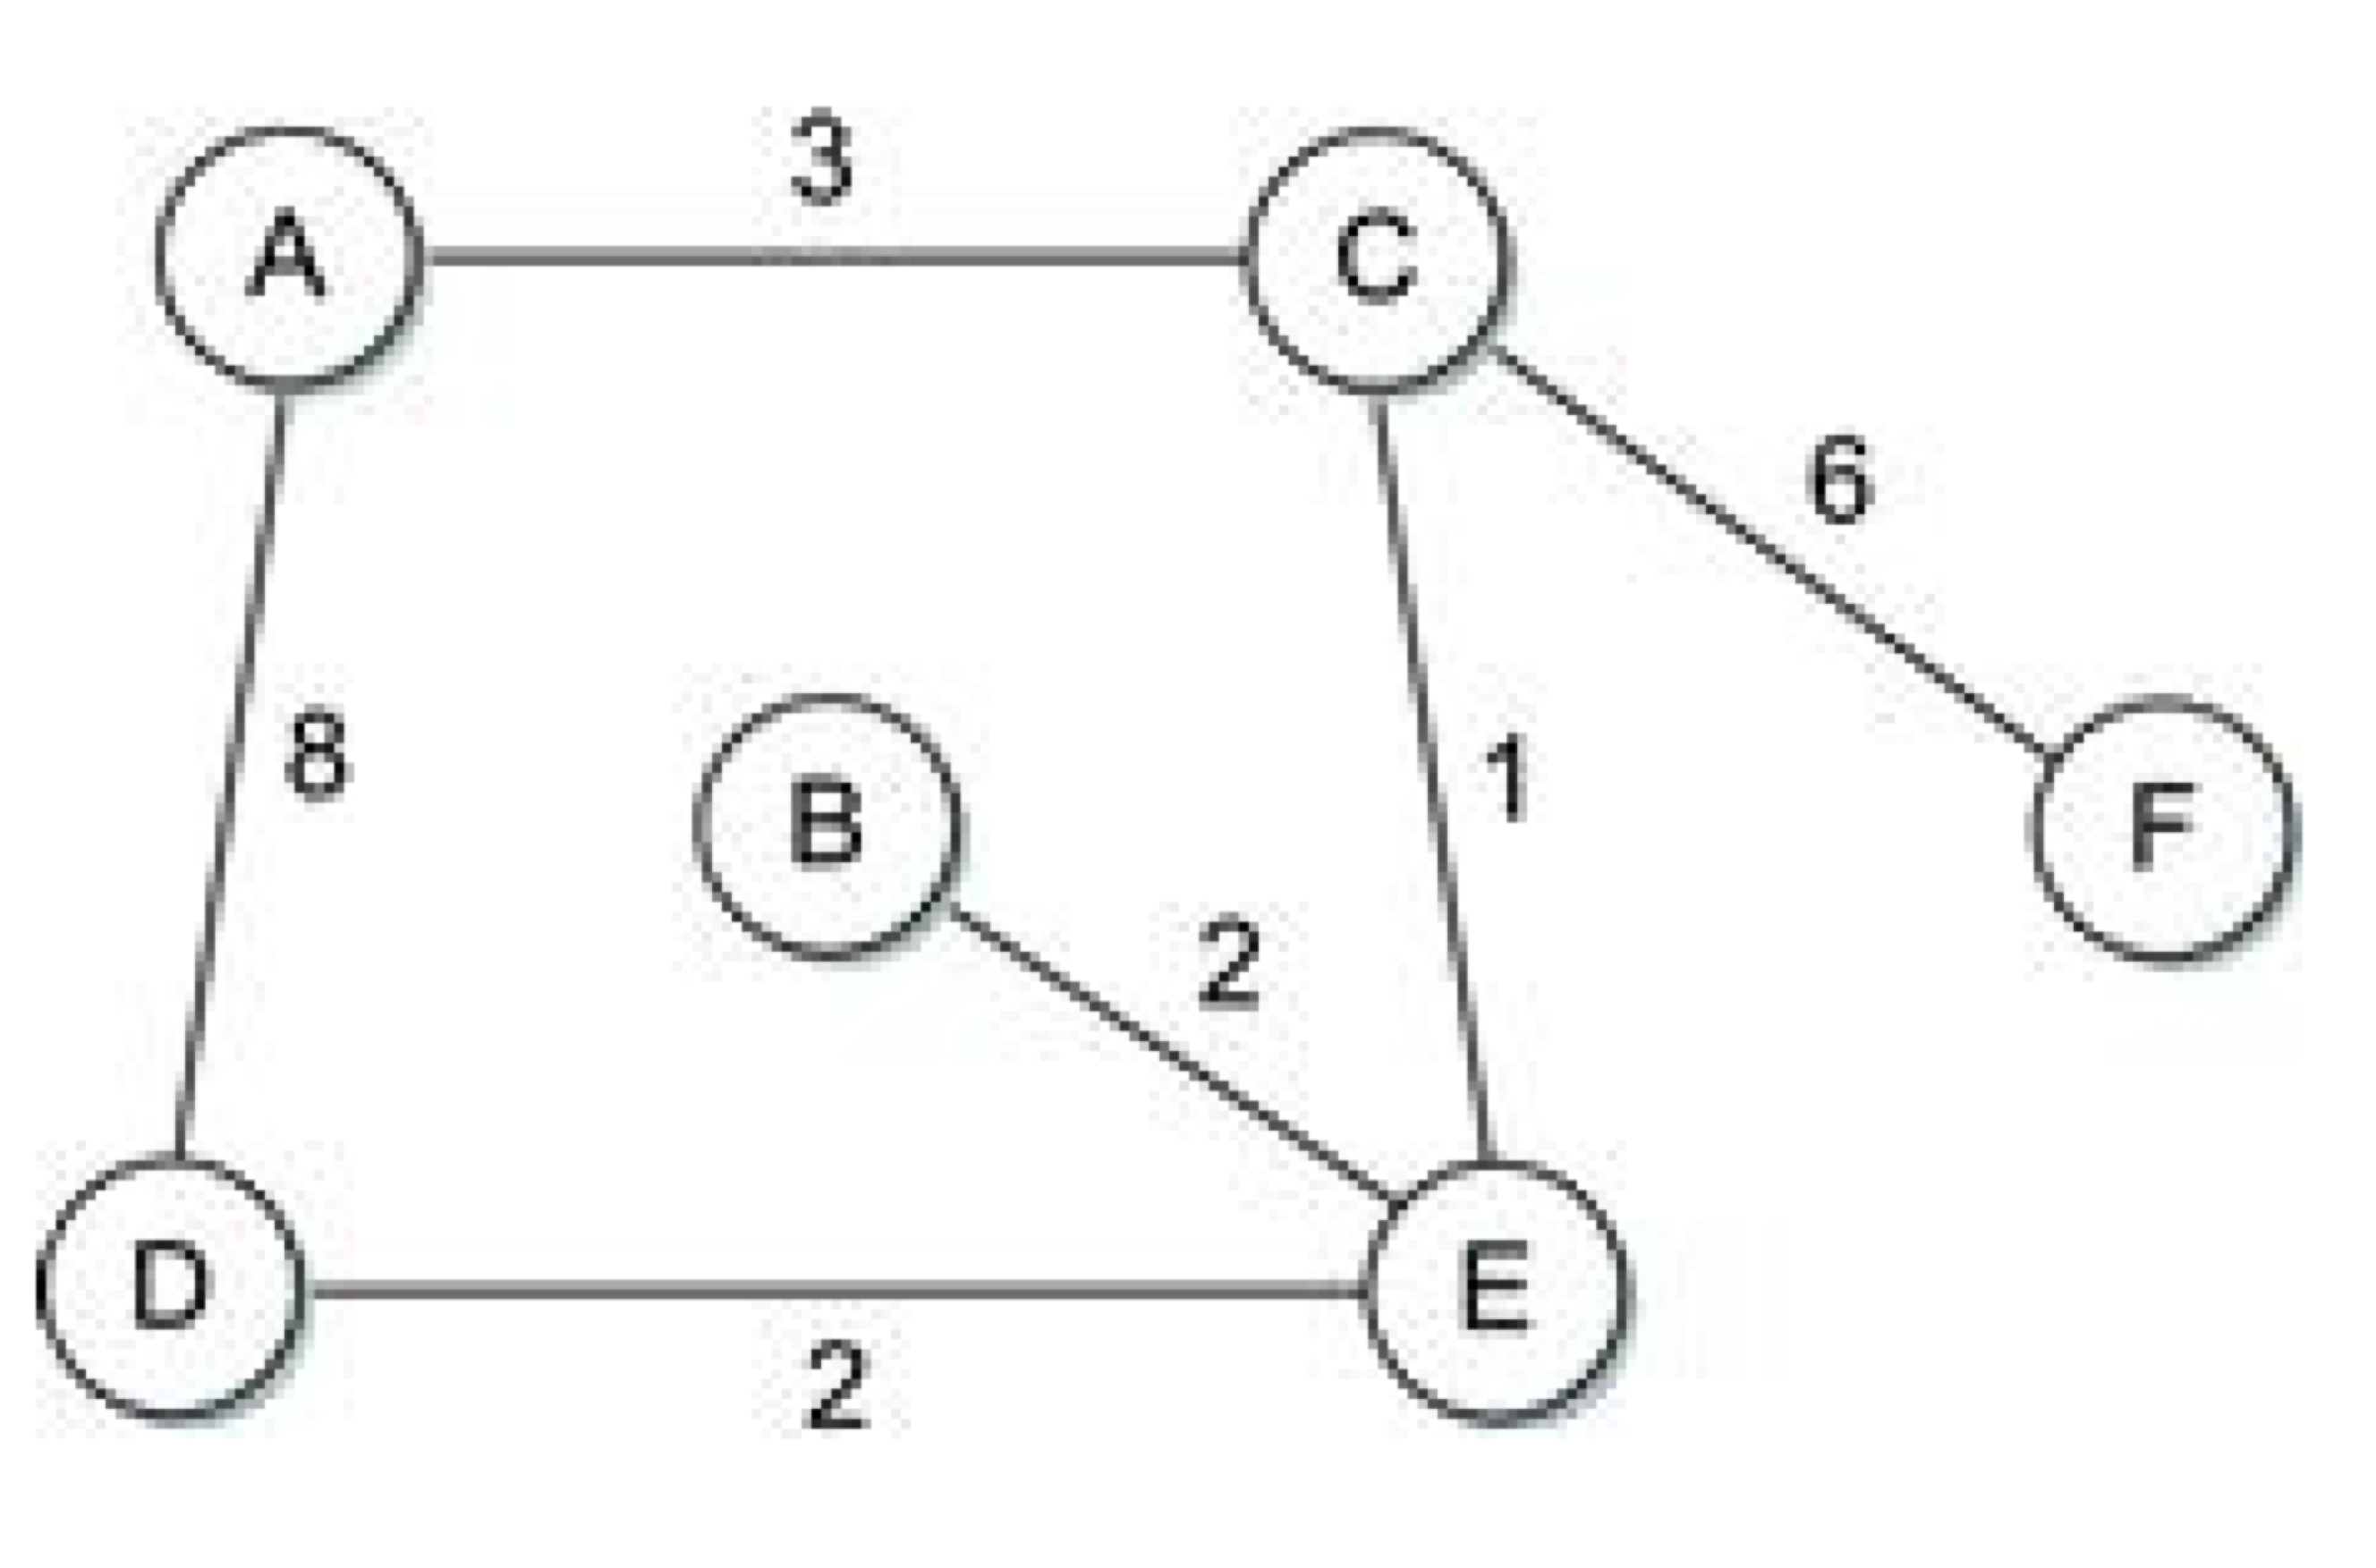
\includegraphics[width=0.4\linewidth]{fig/vector.png}
\end{center}
\begin{parts}
\part[4] Step 1: each node knows only the distances to its immediate neighbors.
\begin{solution}
	See Table 3 part a below
\end{solution}
\part[6] Step 2: each node has reported its distance vector from part (a) to it's neighbors and updated.
\begin{solution}
		See Table 3 part b above
\end{solution}
\part[6] Step 3: each node has reported its distance vector from part (b) to it's neighbors and updates.
\begin{solution}
			See Table 3 part c below
\end{solution}

\end{parts}
% 7.a
\begin{table}[]
	\centering
	\caption{Part a}
	\label{Solution 7}
	\begin{tabular}{|c|c|c|c|c|c|c|}
		\hline
		\multicolumn{7}{|c|}{Distance, Next Hop to Reach Node}              \\ \hline
		& A        & B        & C        & D        & E        & F        \\ \hline
		A & 0        & $\infty$ & 3 (C)    & 8 (D)    & $\infty$ & $\infty$ \\
		B & $\infty$ & 0        & $\infty$ & $\infty$ & 2 (E)    & $\infty$ \\
		C & 3 (A)    & $\infty$ & 0        & $\infty$ & 1 (E)    & 6 (F)    \\
		D & 8 (A)    & $\infty$ & $\infty$ & 0        & 2 (E)    & $\infty$ \\
		E & $\infty$ & 2 (B)    & 1 (C)    & 2 (D)    & 0        & $\infty$ \\
		F & $\infty$ & $\infty$ & 6 (C)    & $\infty$ & $\infty$ & 0       
	\end{tabular}
\end{table}
% 7.b
\begin{table}[]
	\centering
	\caption{Part b}
	\label{Solution 7}
	\begin{tabular}{|c|c|c|c|c|c|c|}
		\hline
		\multicolumn{7}{|c|}{Distance, Next Hop to Reach Node}        \\ \hline
		& A        & B        & C     & D        & E     & F        \\ \hline
		A & 0        & $\infty$ & 3 (C) & 8 (D)    & 4 (C) & 9 (C)    \\
		B & $\infty$ & 0        & 3 (E) & 4 (E)    & 2 (E) & $\infty$ \\
		C & 3 (A)    & 3 (E)    & 0     & 3 (E)    & 1 (E) & 6 (F)    \\
		D & 8 (A)    & 4 (E)    & 3 (E) & 0        & 2 (E) & $\infty$ \\
		E & 4 (C)    & 2 (B)    & 1 (C) & 2 (D)    & 0     & 7 (C)    \\
		F & 9 (C)    & $\infty$ & 6 (C) & $\infty$ & 7 (C) & 0       
	\end{tabular}
\end{table}
% 7.c
\begin{table}[]
	\centering
	\caption{Part c}
	\label{Solution 7}
	\begin{tabular}{|c|c|c|c|c|c|c|}
		\hline
		\multicolumn{7}{|c|}{Distance, Next Hop to Reach Node} \\ \hline
		& A      & B      & C      & D      & E     & F     \\ \hline
		A  & 0      & 6 (C)  & 3 (C)  & 8 (D)  & 4 (C) & 9 (C) \\
		B  & 6 (C)  & 0      & 3 (E)  & 4 (E)  & 2 (E) & 9 (E) \\
		C  & 3 (A)  & 3 (E)  & 0      & 3 (E)  & 1 (E) & 6 (F) \\
		D  & 8 (A)  & 4 (E)  & 3 (E)  & 0      & 2 (E) & 9 (E) \\
		E  & 4 (C)  & 2 (B)  & 1 (C)  & 2 (D)  & 0     & 7 (C) \\
		F  & 9 (C)  & 9 (E)  & 6 (C)  & 9 (E)  & 7 (C) & 0    
	\end{tabular}
\end{table}

\newpage

\question Suppose the network from the previous problem has been upgraded to use Link State routing.
\begin{parts}
\part[4] Show the information sent out as part of the link state for each host.
\begin{solution}
	% This is not worth the 3 hours it would take to write out.
\end{solution}
\part[10] Run the forward search algorithm (not Dijkstra's search) for node C. Make sure you check your final answer against the network to ensure you arrived at the correct forwarding decisions. You should assume that all of the link state packets have been flooded through the network.
\begin{solution}
	% see previous
\end{solution}
\end{parts}

\question[6] A particular organization is given the CIDR address range 210.81.112/20. What are all of the addresses owned by this organization? (List them as ranges, not individual values)
\begin{solution}
	 210.81.112.0 - 210.81.127.255 
\end{solution}

\question A simple CIDR routing table is shown below. For each address, indicate which entry in the table it matches.
\begin{center}
\begin{tabularx}{0.3\linewidth}{>{\centering\arraybackslash}Xc}
\toprule
\emph{Address Mask} & \emph{Port} \\
\midrule
10.19.0.0/16 & 1 \\ %  10.19.0.0 - 10.19.255.255 
10.19.128/17 & 2 \\ %  10.19.128.0 - 10.19.255.255 
10.19.192/18 & 3 \\ %  10.19.192.0 - 10.19.255.255 
10.19.192/19 & 4 \\ %  10.19.192.0 - 10.19.223.255 
0.0.0.0/1    & 5 \\ %  0.0.0.0 - 127.255.255.255 
1.0.0.0/1    & 6 \\ %  0.0.0.0 - 127.255.255.255 
\bottomrule
\end{tabularx}
\end{center}
\begin{parts}
\part[2] 141.219.2.10
\begin{solution}
	None.
	Port 5 and 6 are closest, but they both are through $ 0.0.0.0 - 127.255.255.255 $.
	A 0 mask would be required for this.
\end{solution}
\part[2] 10.10.10.10
\begin{solution}
	Port 5 and Port 6, Port 5 preferably since it comes first on the list.
\end{solution}
\part[2] 10.19.86.141
\begin{solution}
	Port 1, Port 5, and Port 6; Port 1 preferably since it comes first on the list.
\end{solution}
\part[2] 10.19.193.6
\begin{solution}
	Port 3, Port 4, Port 5, and Port 6; Port 3 preferably since it comes first on the list.
\end{solution}
\part[2] 10.19.255.86
\begin{solution}
	Port 2, Port 3, Port 5, and Port 6; Port 2 preferably since it comes first on the list.
\end{solution}
\part[2] 10.19.192.18
\begin{solution}
	Port 3, Port 4, Port 5, and Port 6; Port 3 preferably since it comes first on the list.
\end{solution}
\end{parts}


\question[8] Explain the software-defined networking approach to separating the routing and forwarding behavior. Why does it possibly lead to better routing decisions?
\begin{solution}
	SDN may lead to better routing decisions as it has much more capability to fix it's own network routing by determining which links have better priorities, better timeouts, ability to create better and more well defined NATs, meter processing, and able to drastically rewrite packets.
\end{solution}


\end{questions}
\end{document}
